\paragraph{QuizziPedia::Front-End::Controllers::TrainingController}
\begin{figure} [ht]
	\centering
	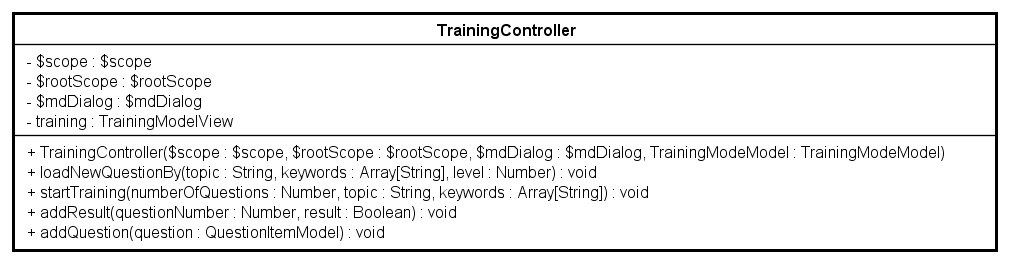
\includegraphics[scale=0.45]{UML/Classi/Front-End/QuizziPedia_Front-end_Controller_TrainingController.png}
	\caption{QuizziPedia::Front-End::Controllers::TrainingController}
\end{figure} \FloatBarrier
\begin{itemize}
	\item \textbf{Descrizione}: questa classe permette di gestire la modalità allenamento sottoponendo all'utente le giuste domande adatte al suo livello;
	\item \textbf{Utilizzo}: fornisce le funzionalità per recuperare le domande che siano in accordo con il livello dell'utente;
	\item \textbf{Relazione con altre classi}:
	\begin{itemize}
		\item \textit{IN} \texttt{TrainingModelView}: ;
		\item \textit{IN} \texttt{TrainingModeModel}: ;
		\item \textit{IN} \texttt{TrainingSetUpTemplate}: rappresenta il componente grafico che permette all'utente di selezionare l'argomento e le parole chiave per iniziare un allenamento con queste caratteristiche. Viene gestito dinamicamente all'interno della view TrainingView attraverso il controller TrainingController;
		\item \textit{IN} \texttt{QuestionController}: ;
		\item \textit{IN} \texttt{QuestionItemMode}: ;
	\end{itemize}
	\item \textbf{Attributi}:
	\begin{itemize}
		\item \texttt{-} \texttt{\$scope: \$scope} \\
		Campo dati contenente un riferimento all’oggetto \$scope creato da \textit{Angular\ped{G}}, viene utilizzato come mezzo di comunicazione tra il controller e la view. Contiene gli oggetti che definiscono il model dell’applicazione;
		\item \texttt{-} \texttt{\$rootScope: \$rootScope} \\
		Campo dati contenente il riferimento all'oggetto globale \$rootScope creato da \textit{Angular\ped{G}}. Viene utilizzato per rendere accessibile a tutti i controller e a tutte le view l'oggetto \texttt{TrainingModeModel}. In questo caso viene utilizzato per inserire in \$rootScope l'oggetto di ritorno della chiamata a \texttt{getNextQuestion};
		\item \texttt{-} \texttt{\$mdDialog: \$mdDialog} \\
		Campo dati contenente un riferimento al servizio della libreria \textit{Material for Angular\ped{G}} che permette di creare delle componenti a popup;
		\item \texttt{+} \texttt{training: TrainingModelView} \\
		Oggetto di tipo \texttt{TrainingModelView}. All'interno di esso sono presenti le variabili e i metodi necessari per il \textit{Two-Way Data-Binding\ped{G}} tra la view \texttt{TrainingView} e il controller \texttt{TrainingController};
	\end{itemize}
	\item \textbf{Metodi}:
	\begin{itemize}
		\item \texttt{+} \texttt{TrainingController(\$scope: \$scope, \$rootscope: \$rootscope, \$mdDialog: \$mdDialog)} \\ Metodo costruttore della classe; \\
		\textbf{Parametri:}
		\begin{itemize}
			\item \texttt{\$scope: \$scope} \\
			Parametro contenente un riferimento all’oggetto \$scope creato da \textit{Angular\ped{G}}. Viene utilizzato come mezzo di comunicazione tra il controller e la view. Contiene gli oggetti che definiscono il viewmodel e il model dell’applicazione;
			\item \texttt{\$rootscope: \$rootscope}\\
			Parametro contenente il riferimento all'oggetto globale \$rootScope creato da \textit{Angular\ped{G}}. Viene utilizzato per rendere accessibile a tutti i controller e a tutte le view l'oggetto \texttt{UserDetailsModel}. In questo caso viene utilizzato per aggiornare in \$rootScope l'oggetto che rappresenta l'utente autenticato all'interno dell'applicazione;
			\item \texttt{\$mdDialog: \$mdDialog} \\
			Parametro contenente un riferimento al servizio della libreria \textit{Material for Angular\ped{G}} che permette di creare delle componenti a popup.
		\end{itemize}
		\item \texttt{-} \texttt{getNextQuestion(): QuestionItemModel} \\ Metodo che gestisce l'evento del click al pulsante "prossima domanda", fa una richiesta al QuestionsController che ritornerà la domanda successiva. Questa domanda andrà salvata nel TrainingModeModel nello \$scope.
	\end{itemize}
\end{itemize}

